\chapter{Fase preliminare alla realizzazione del progetto}
\thispagestyle{empty}

Prima della realizzazione del progetto per controllare entrambi gli strumenti, si � optato per la scrittura di due progetti separati. In questo modo � stato possibile verificare la versione del codice pi� efficacie per ogni strumento, cos� da poter unire in seguito le due logiche, evitando conflitti.

\section{Fotocamera}

Per entrare in confidenza con il linguaggio di programmazione grafico LabVIEW e con lo strumento, si � reso necessario partire da un esempio fornito con le API LabVIEW legate alla nuova fotocamera intensificata.

\subsection{Breve descrizione dello strumento}
La fotocamera intensificata per cui si deve scrivere il programma che la controlli � la 4 Picos con CCD intensificato di Stanford Computer Optics, Inc.

\subsection{Descrizione dell'esempio fornito}

L'esempio fornito � molto semplice e non contiene tutte le opzioni disponibili per la fotocamera. Analizziamo come fatto in precedenza i due componenti principali del programma: front panel e block diagram.

\subsubsection{Front Panel}
\begin{figure} [h]
	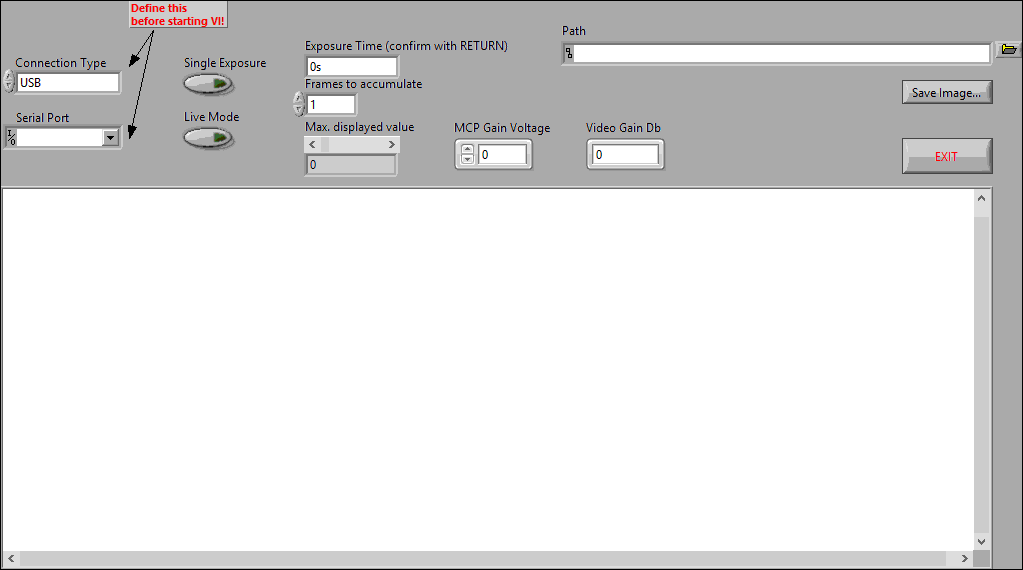
\includegraphics[width=\linewidth]{img/SCOexample_fp.png}
	\caption{Front Panel del progetto per sola fotocamera}
	\label{fig:midProj_camera_fp}
\end{figure}
Nel front panel in figura \ref{fig:midProj_camera_fp} possiamo vedere due controlli che � obbligatorio definire prima della partenza del VI, e sono il tipo di connessione \textit{Connection Type} e la porta seriale \textit{Serial Port} nel caso in cui il tipo di connessione sia \textit{Analog}. � infatti permesso scegliere fra tre tipi di connessione allo strumento: \textit{USB} (che � la connessione usata nel nostro caso), \textit{CameraLink} o \textit{Analog}. A fianco di questi due controlli troviamo due bottoni booleani per acquisire immagini in un singolo frame oppure in modo continuo. � poi possibile inserire il tempo di esposizione \textit{Exposure Time}, il numero di frame da catturare \textit{Frames to accumulate}, e modificare il valore \textit{Max. displayed value} del fondo scala. Un indicatore di immagine rende possibile la visualizzazione dell'immagine e un bottone booleano permette di salvare l'immagine. Infine troviamo un controllo per terminare il programma.

\subsubsection{Block Diagram}
\begin{figure} [h]
	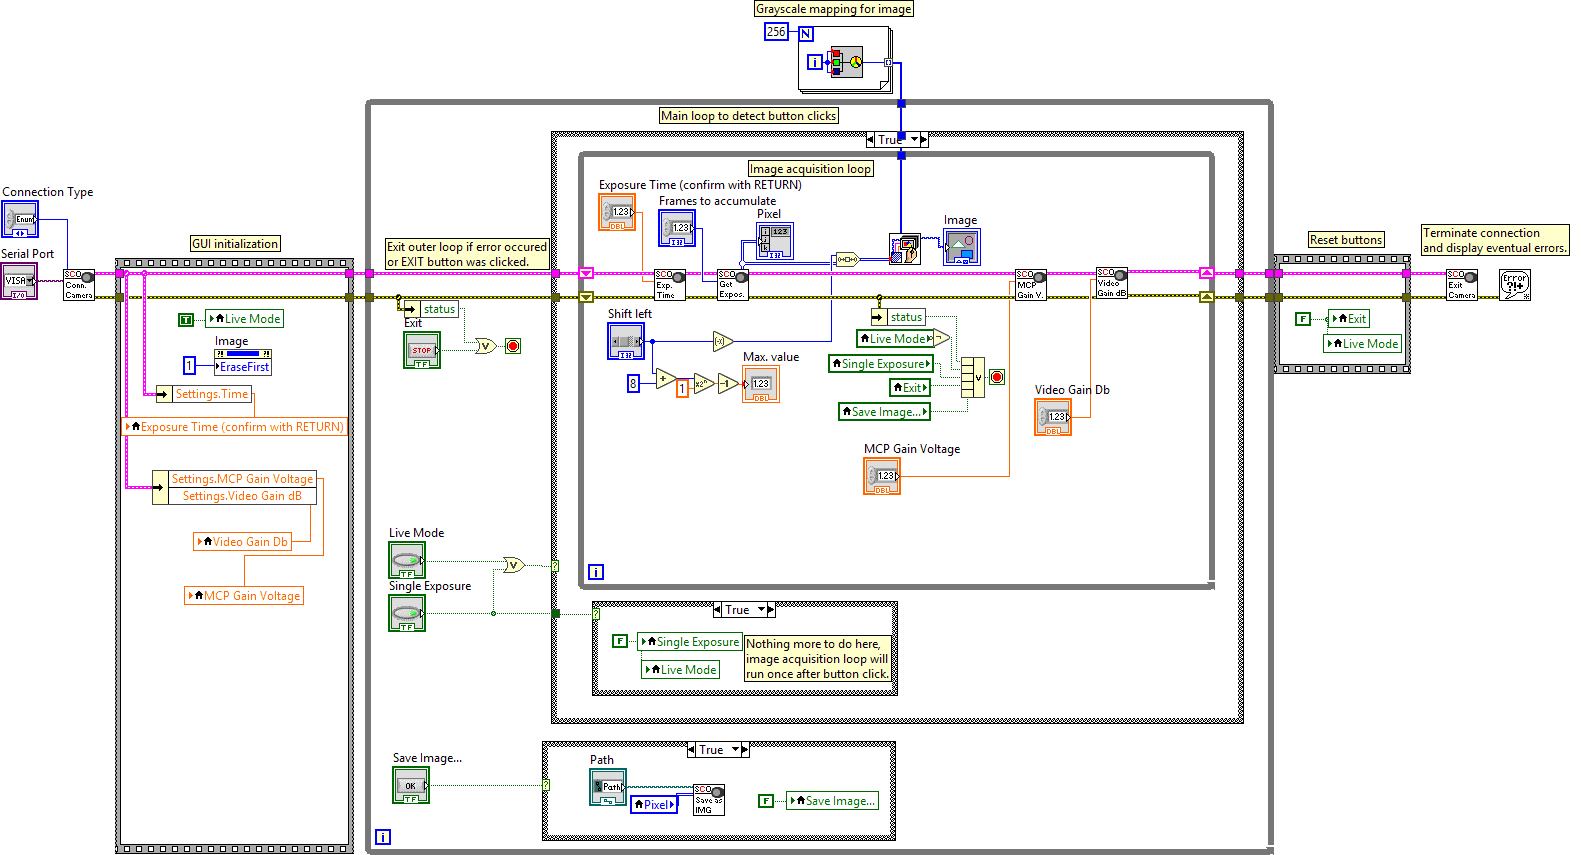
\includegraphics[width=\linewidth]{img/SCOexample_bd.png}
	\caption{Block Diagram del progetto per sola fotocamera}
	\label{fig:midProj_camera_bd}
\end{figure}
Si pu� considerare il bock diagram, in figura \ref{fig:midProj_camera_bd}, idealmente diviso in tre parti che eseguono in senquenza: una parte iniziale di inizializzazione, una intermedia di funzionamento del programma, e una finale di chiusura graceful dell'applicazione.\\
Il primo subVI invocato � \emph{ConnectCamera.vi} e deve essere invocato prima che la fotocamera sia utilizzata, imposta la connessione della fotocamera dipendentemente dall'input immesso dall'utente; restituisce in uscita un cluster contenente tutte le informazioni che riguardano le impostazioni della fotocamera. Tale cluster di dati, insieme al cluster di errore, entra in una flat sequence che recupera le impostazioni memorizzate da un uso antecedente dello strumento e le mostra nel controlli appositi nel front panel; viene anche impostato il bottone booleano \textit{Live Mode} a false.\\
In seguito alla flat sequence troviamo un ciclo while con lo scopo di individuare il cambiamento dei bottoni e dei controlli. All'interno di questo ciclo sono presenti due case structure: la prima associata al bottone \textit{Save Image...} che permette di salvare l'immagine, la seconda associata all'\textit{or} fra il valore dei due bottoni \textit{Single Exposure} e \textit{Live Mode}. Viene eseguito quindi il codice all'interno di quest'ultima case structure qualora o un bottone o l'altro esclusivamente (grazie ad un'altra case structure interna) abbiamo il valore true. Una volta dentro la case structure viene eseguito un ciclo while all'interno del quale vengono invocate alcune API LabVIEW della fotocamera: dapprima \emph{SetExposureTime.vi} con la quale si setta il tempo di esposizione, poi \emph{GetExposure.vi} che restituisce la matrice di pixel corrispondente alla foto. Attraverso alcuni calcoli che tengono in considerazione anche il valore di fondo scala inserito viene generata l'immagine da visualizzare del controllo destinato. Il ciclo while interno si arresta se viene presa una singola immagine, oppure se non si � selezionata la modalit� Live Mode, o se si � premuto il bottone \textit{Exit} per uscire dal ciclo o quello di salvataggio dell'immagino, o ancora se si � verificato qualche errore. Il ciclo esterno si arresta invece se si � verificato qualche errore o se si � invocato il bottone \textit{Exit} per fermarlo.\\
All'esterno di tale ciclo viene eseguito l'ultimo frammento di codice: in una flat sequence vengono resettati i bottoni di \textit{Exit} e \textit{Live Mode}, impostandoli a false, e infine viene invocato l'ultimo subVI relativo alla fotocamera, \emph{ExitCamera.vi}, che ha il compito di rilasciare le risorse impegnate dal programma e arrestare la fotocamera nel modo corretto.

\section{Monocromatore}
Ad un primo tentativo di refactoring del progetto preesistente il codice relativo al controllo del monocromatore si � rivelato troppo caotico e sparso. Per questo si � realizzato un nuovo programma, prendendo ovviamente spunto dal precedente, dedicato solo al monocromatore, che rispettasse il corretto flusso dei dati e non facesse uso di flat sequence. Si descrivono di seguito front panel e block diagram di tale programma.

\subsection{Front Panel}
\begin{figure} [h]
	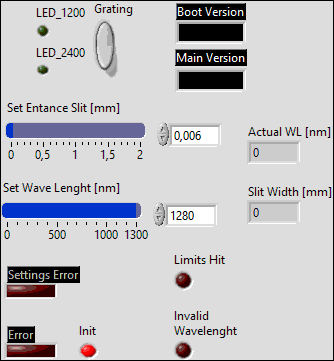
\includegraphics[width=0.5\linewidth]{img/ControlOnlyMono_Refactored.png}
	\caption{Front Panel del progetto per solo monocromatore}
	\label{fig:midProj_mono_fp}
\end{figure}
Gli elementi presenti nel front panel in figura \ref{fig:midProj_mono_fp} sono gli stessi dedicati al monocromatore nel precedente progetto, li rivedremo comunque brevemente. I controlli presenti sono:
\begin{itemize}
	\item \textit{Grating} per distinguere il tipo ti grating (1200 o 2400)
	\item \textit{Set Entrance Slit} per impostare la slit di entrata
	\item \textit{Set Wave Length} per inserire la lunghezza d'onda desiderata
\end{itemize}
Mentre gli indicatori sono:
\begin{itemize}
	\item \textit{Init} led che segnala se il monocromatore � stato inizializzato correttamente
	\item \textit{Error} led che segnala la presenza di eventuali errori in fase di inizializzazione
	\item \textit{Boot/Main Version} informazioni sulla versione del programma in uso
	\item \textit{Actual WL} lunghezza d'onda effettiva inserita
	\item \textit{Slit Width} slit di entrata inserita
	\item \textit{Settings Error} led che segnala un eventuale errore generico nel settaggio delle impostazioni del monocromatore
	\item \textit{Limits Hit} led che segnala l'inserimento di una lunghezza d'onda troppo alta
	\item \textit{Invalid Wavelength} led che segnala l'inserimento di una lunghezza d'onda non valida
\end{itemize}

\subsection{Block Diagram}
\begin{figure} [h]
	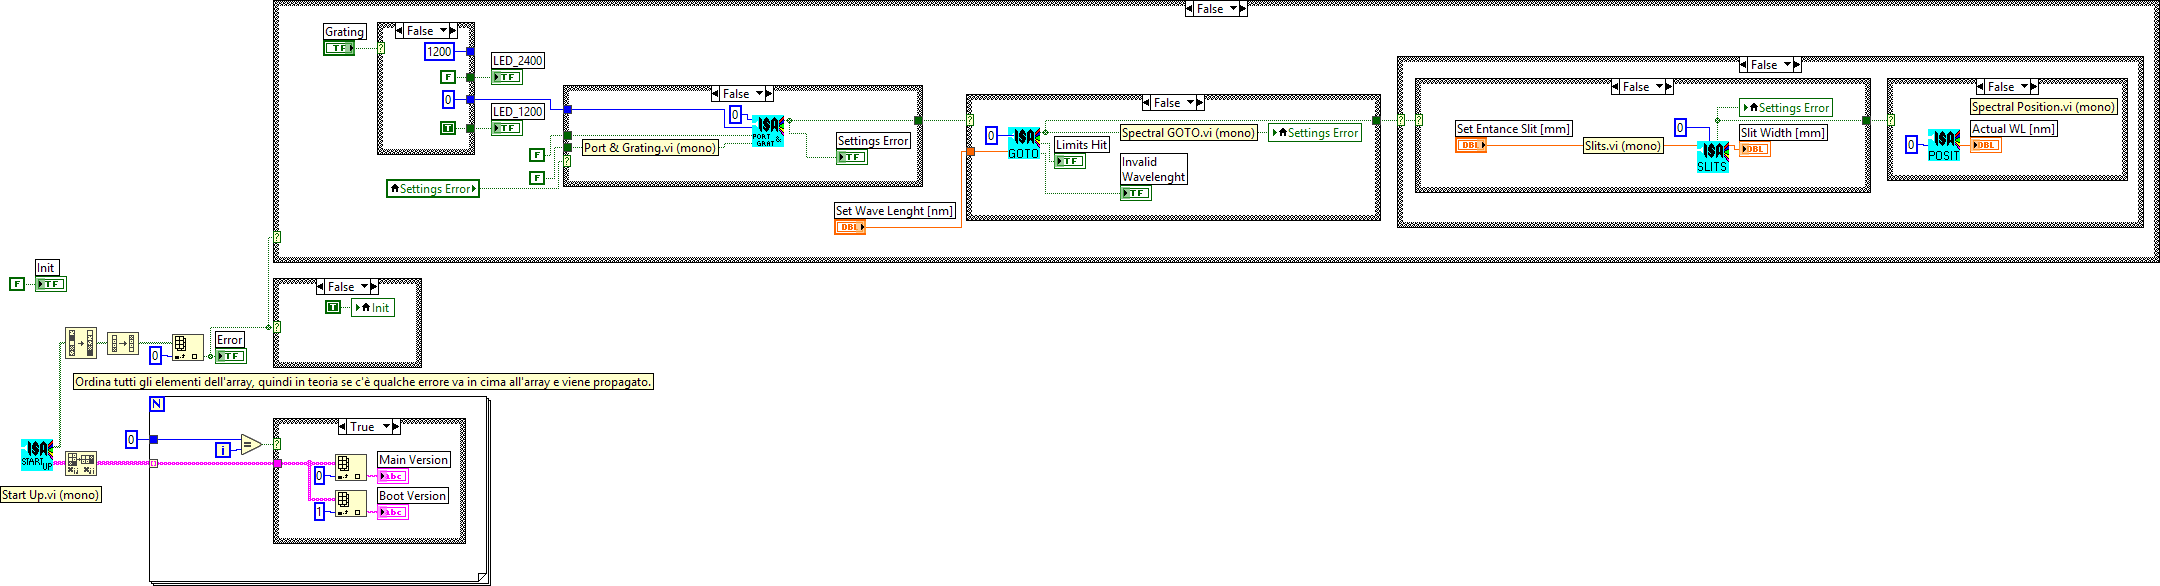
\includegraphics[width=\linewidth]{img/ControlOnlyMono_Refactored_bd.png}
	\caption{Block Diagram del progetto per solo monocromatore}
	\label{fig:midProj_mono_bd}
\end{figure}
Per la realizzazione del block diagram in figura \ref{fig:midProj_mono_bd} si � chiaramente preso spunto da quello gi� esistente, ma si � impiegato un consistente refactoring in particolare per eliminare le flat sequence.\\
Il primo subVI ad essere invocato � \emph{Start Up.vi} che porta i componenti interni del monocromatore nella posizione di default e restituisce il numero di versione del programma. Tale subVI restituisce anche un array di errori: esso viene ordinato in ordine crescente e ne viene estratto l'elemento in cima, se vi � un errore allora non � possibile continuare con il programma, in caso contrario si pu� procedere. Si entra quindi (in assenza di errori) nella case structure che permette di impostare come si desidera il monocromatore. I subVI che vengono invocati, in sequenza, sono: \emph{Port \& Grating.vi} per specificare il grating, \emph{Spectral GOTO.vi} per portare gli elementi interni alla lunghezza d'onda inserita dall'utente, \emph{Slits.vi} per inserire la slit di entrata e \emph{Spectral Position.vi} per completare gli indicatori corrispondenti. Chiaramente ognuno di questi subVI � inserito all'interno di una case structure e verrano eseguiti solo qualora il subVI precedente non abbia restituito in uscita errori. In questo modo si eliminano completamente le flat sequence e si sfrutta l'andamento del flusso dei dati.